\documentclass{standalone}
\usepackage{graphicx}	
\usepackage{amssymb, amsmath}
\usepackage{color}

\usepackage{tikz}
\usetikzlibrary{intersections, backgrounds}
\usepackage{pgfmath}

\definecolor{light}{RGB}{220, 188, 188}
\definecolor{mid}{RGB}{185, 124, 124}
\definecolor{dark}{RGB}{143, 39, 39}
\definecolor{highlight}{RGB}{180, 31, 180}
\definecolor{gray10}{gray}{0.1}
\definecolor{gray20}{gray}{0.2}
\definecolor{gray30}{gray}{0.3}
\definecolor{gray40}{gray}{0.4}
\definecolor{gray60}{gray}{0.6}
\definecolor{gray70}{gray}{0.7}
\definecolor{gray80}{gray}{0.8}
\definecolor{gray90}{gray}{0.9}
\definecolor{gray95}{gray}{0.95}

\newcommand*{\offset}{0.025}

\begin{document}

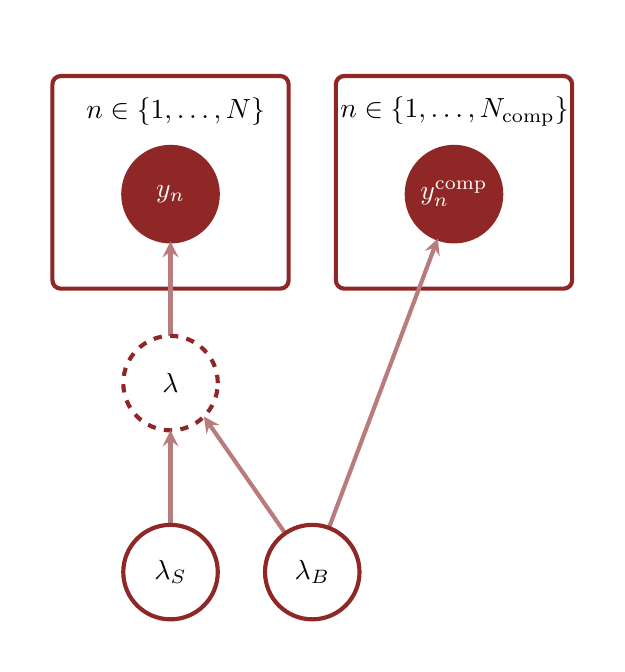
\begin{tikzpicture}[scale=0.3, thick]

\pgfmathsetmacro{\r}{2}

% Two
\pgfmathsetmacro{\dx}{30}
\pgfmathsetmacro{\dy}{0}

\draw[white] (-6 + \dx, -15 + \dy) rectangle (18 + \dx, 11 + \dy);

\filldraw[fill=white, draw=dark, line width=1.5, rounded corners=3pt] (-5 + \dx, 0 + \dy) rectangle (5 + \dx, 9 + \dy);

\node[right] at (-4 + \dx, 7.5 + \dy) { $n \in \{1, \ldots, N\}$ };

\filldraw[fill=dark, draw=dark, line width=1.5] (0 + \dx, 4 + \dy) circle (\r)
node[color=white] { $y_{n}$ };

\filldraw[fill=white, draw=dark, line width=1.5, rounded corners=3pt] (7 + \dx, 0 + \dy) rectangle (17 + \dx, 9 + \dy);

\node[right] at (6.75 + \dx, 7.5 + \dy) { $n \in \{1, \ldots, N_{\text{comp}}\}$ };

\filldraw[fill=dark, draw=dark, line width=1.5] (12 + \dx, 4 + \dy) circle (\r)
node[color=white] { $y^{\text{comp}}_{n}$ };

\draw[->, >=stealth, color=mid, line width=1.5] (0 + \dx, -4 + \dy) -- (0 + \dx, 4 - \r + \dy);

\filldraw[fill=white, draw=dark, dashed, line width=1.5] (0 + \dx, -4 + \dy) circle (\r)
node[color=black] { $\lambda$ };

\draw[->, >=stealth, color=mid, line width=1.5] (0 + \dx, -12 + \dy) -- (0 + \dx, -4 - \r + \dy);

\filldraw[fill=white, draw=dark, line width=1.5] (0 + \dx, -12 + \dy) circle (\r)
node[color=black] { $\lambda_{S}$ };

\draw[->, >=stealth, color=mid, line width=1.5] (6 + \dx, -12 + \dy) -- ({0 + \r * cos(45) + \dx}, {-4 - \r * sin(45) + \dy});

\draw[->, >=stealth, color=mid, line width=1.5] (6 + \dx, -12 + \dy) -- ({12 - \r * cos(70) + \dx}, {4 - \r * sin(70) + \dy});

\filldraw[fill=white, draw=dark, line width=1.5] (6 + \dx, -12 + \dy) circle (\r)
node[color=black] { $\lambda_{B}$ };

\end{tikzpicture}

\end{document}  